\section{Architektur}

\begin{figure}[ht]
	\centering
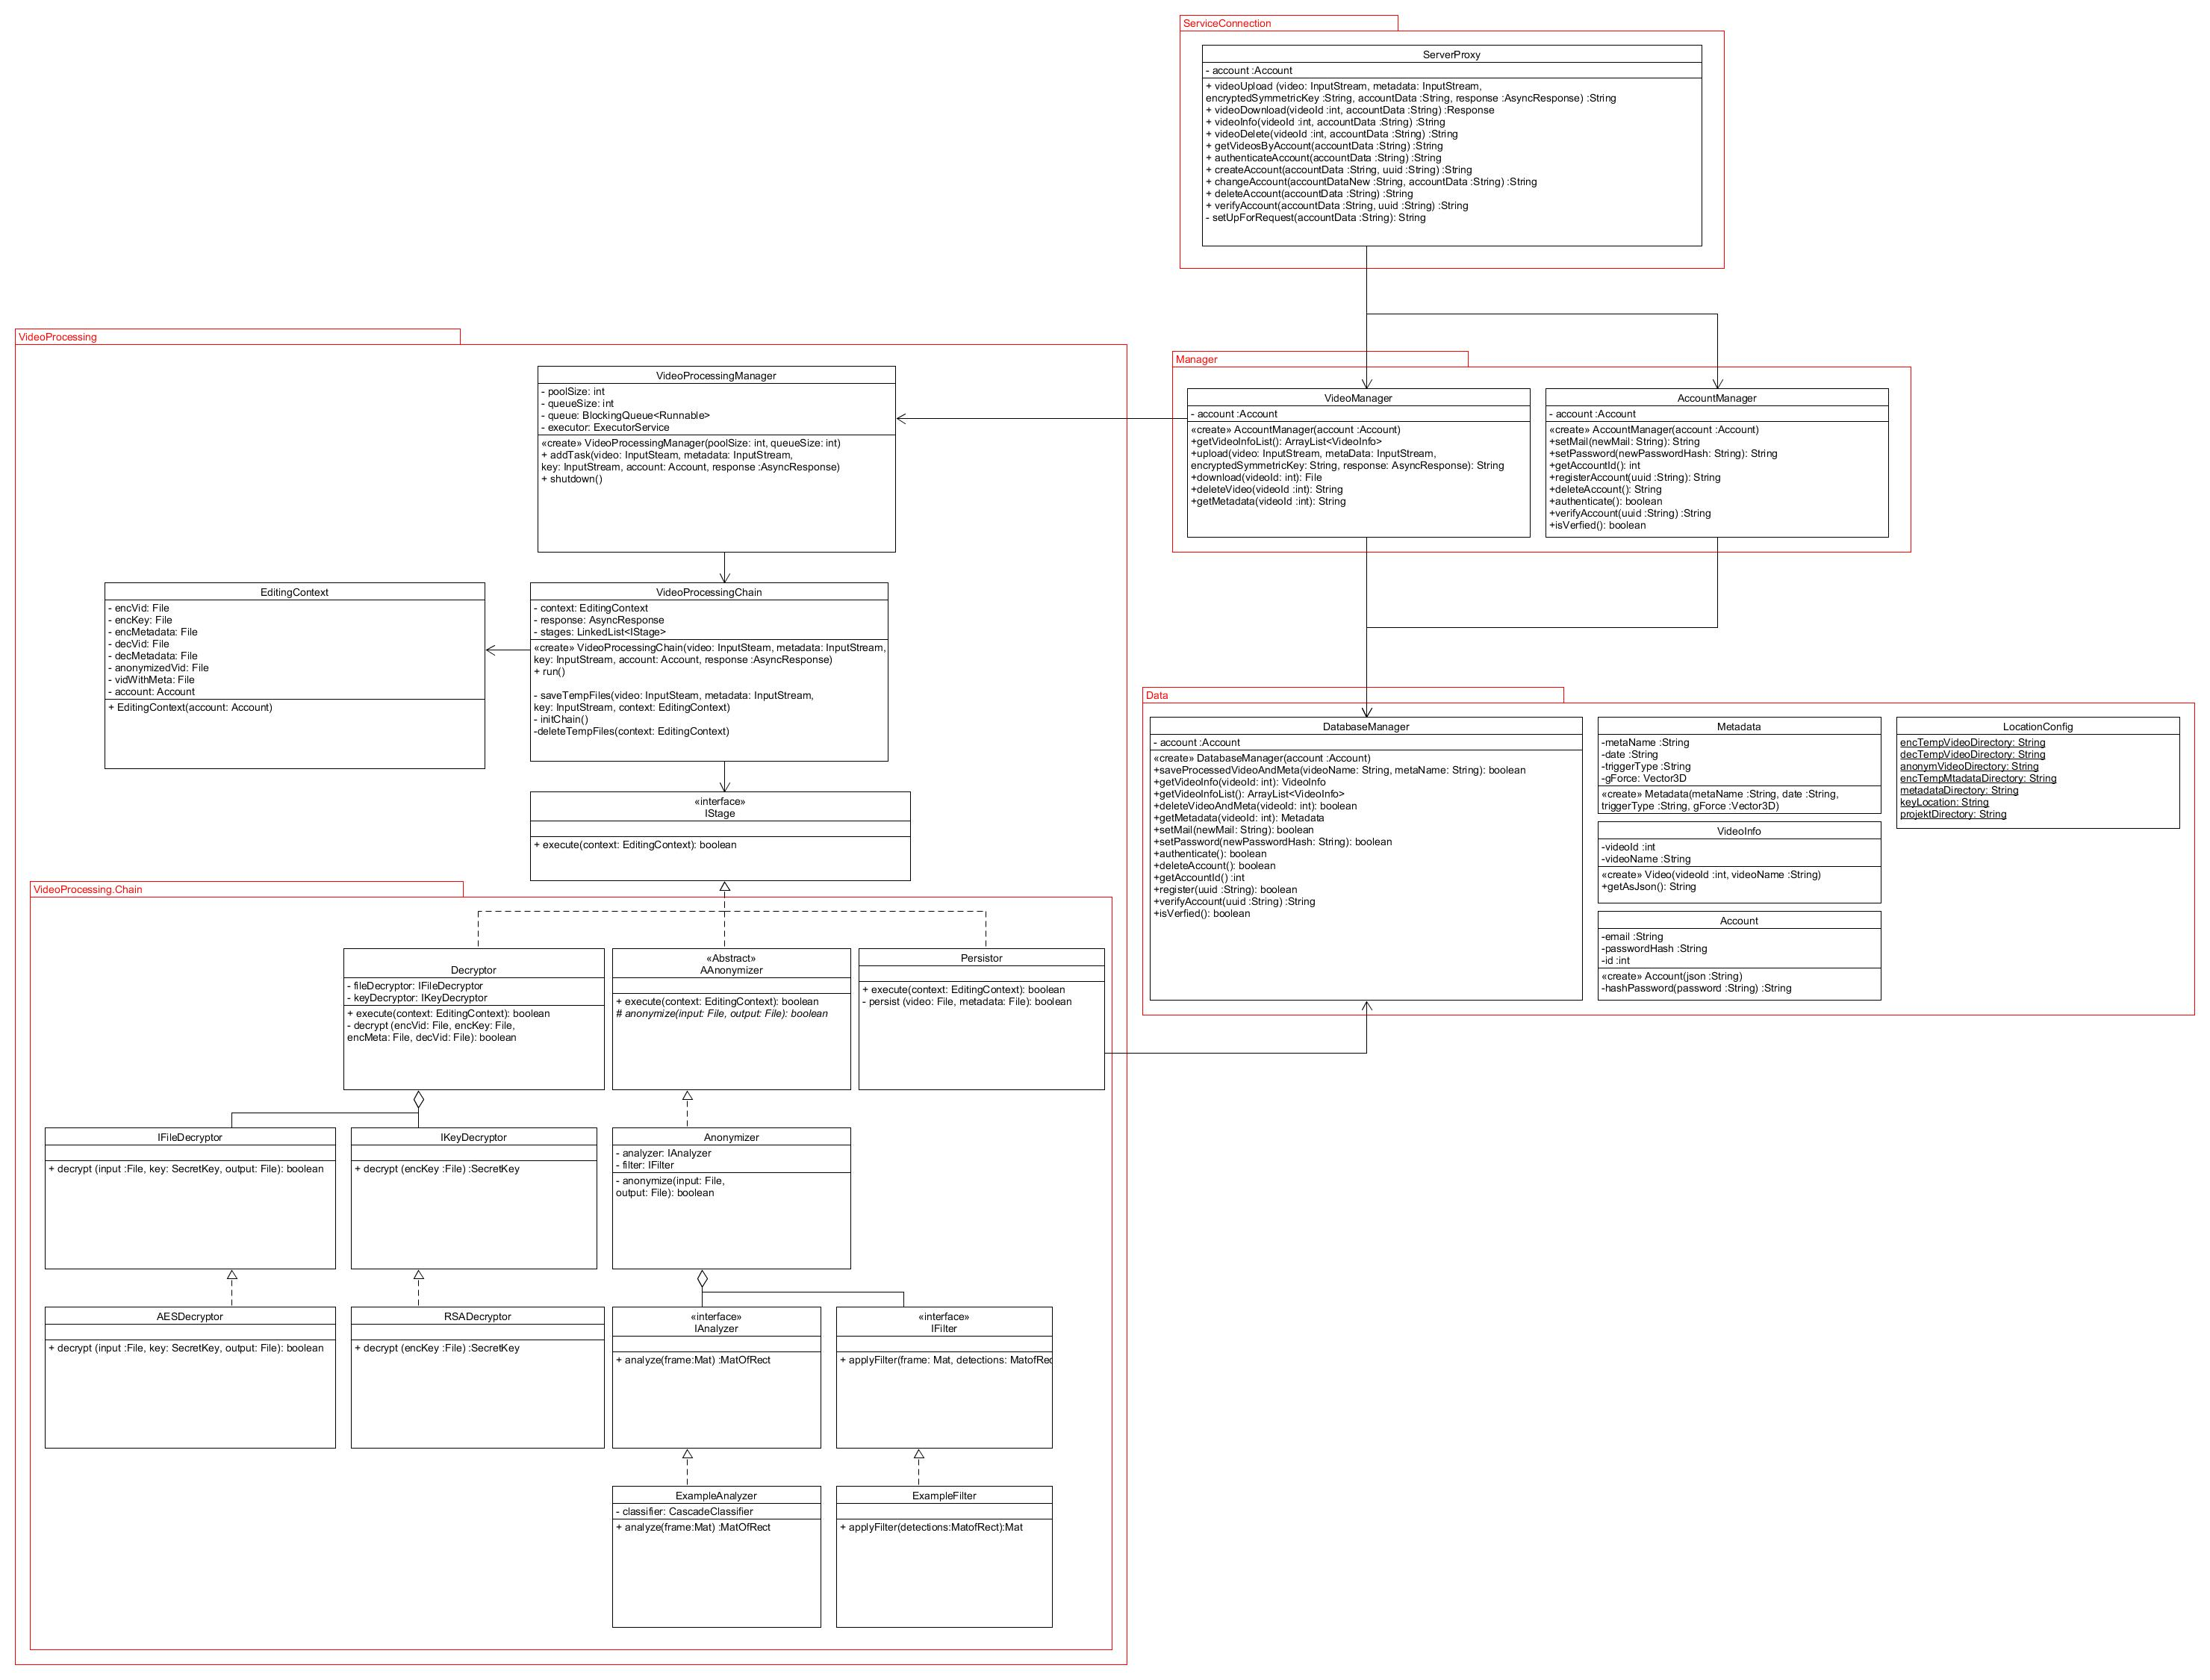
\includegraphics[width=1\textwidth]{./resources/Diagramme/Webservice/UMLSERVERPCC.jpg}
\caption{UML Diagramm des Web-Dienst}
	\label{service:fig:modules_overview}
\end{figure}

\subsection{Multithreading}
Um Anfragen vieler Nutzer unabhängig gleichzeitig zu bearbeiten, nimmt sich der Dienst für jede Anfrage einen einzelnen Thread. Unser verwendeter Webserver Jetty macht dies automatisch, indem er für jede Anfrage einen Thread aus einem internen ThreadPool nimmt, sofern vorhanden.\newline
Da die Bearbeitung der Videos jedoch sehr zeitaufwändig ist, lagern wie die Bearbeitung auf einen eigenen Worker ThreadPool um~\eqref{service:pattern:masterworker}, damit der Anfrage-Thread möglichst schnell seine Arbeit beenden kann und bereit für neue Anfragen ist. 

\subsection{Entwurfsmuster} \label{service:pattern}
Der Web-Service benutzt verschiedene Entwurfsmuster um vor allem zwei Ziele zu erreichen: 1. Eine schnelle und zeitlich unabhängige Bearbeitung von Anfragen und 2. Eine hohe Modularität und Austauschbarkeit.

\subsubsection{Proxy} \label{service:pattern:proxy}
Die Webanbindung des Services wird in dem \nameref{service:klasse:ServerProxy} gekapselt. Der Proxy bearbeitet bzw. verschickt lediglich die Http-Anfragen und leitet alle weitere Arbeit weiter. Dies sorgt für eine höhere Austauschbarkeit, da so die Webanbindung unabhängig von der eigentlichen Bearbeitung der Anfragen ausgetauscht werden kann und umgekehrt.

\subsubsection{Master-Worker} \label{service:pattern:masterworker}
Da die Bearbeitung der Videos auf dem Web-Dienst rechen- und damit zeitintensiv ist, nutzt er einen eigenen Worker-ThreadPool zur Bearbeitung der Videos. Dadurch muss der für die Serveranfrage verwendete Thread nur neues \nameref{service:klasse:VideoProcessingChain}-Objekt erzeugen erzeugen und in die Warteschlange des \nameref{service:klasse:VideoProcessingManager} einreihen. Dann kann dann direkt zurückkehren um neue Anfragen entgegenzunehmen. Dies erlaubt dem Server schneller und mehr externe Anfragen anzunehmen, bevor dieser blockiert.\newline
Der VideoProcessingManager kann dann unabhängig von externen Anfragen auf seine eigenen Worker-Threads verteilen, um die Warteschlange abzuarbeiten.

\subsubsection{Pipeline} \label{service:pattern:pipeline}
Es gibt viele verschiedene Methoden Videos auf personenbezogene Daten zu analysieren. Dabei kann die Anzahl und Reihenfolge der durchlaufenen Arbeitsschritte stark variieren. Um den Web-Dienst in dieser Hinsicht möglichst flexibel zu gestalten, wird das Pipeline-Muster verwendet: \newline
Jeder Arbeitsschritt muss die entheitliche Schnittstelle \nameref{service:klasse:IStage} implementieren und somit eine Methode bereitstellen, die den Arbeitsschritt mithilfe des \nameref{service:klasse:EditingContext} ausführt.\newline
Die \nameref{service:klasse:VideoProcessingChain} besitzt eine Liste von Arbeitsschritten, die sie, sofern keine Fehler entstehen, der Reihe nach ausführt. In diese Liste können jeder Zeit Arbeitsschritte eingefügt bzw. entfernt werden, die Reihenfolge der Arbeitsschritte verändert, oder der komplette Ablauf ausgetauscht werden. Theoretisch sind sogar Änderungen zur Laufzeit möglich.\newline
Durch die Kapselung der Arbeitsschritte in einzelne Klassen ist es zudem möglich Arbeitsschritte in verschiedenen Ausführungsreihenfolgen wiederzuverwenden ohne, dass erneuter Initialisierungsaufwand entsteht.

\subsubsection{Strategie} \label{service:pattern:strategie}
Da es für das, von uns bereitgestellte Bearbeitungschema für Videos, viele verschiedene Algorithmen für die einzelnen Schritte gibt, wird das Strategie-Muster verwendet:\newline
Für die Schritte, die man eventuell austauschen möchte (z.B den Filter mit dem Bildbereiche unkenntlich gemacht werden) existiert eine Schnittstelle (z.B \nameref{service:klasse:IFilter}). Dann können nach belieben konkrete Implementierungen (hier z.B. \nameref{service:klasse:ExampleFilter}) ausgetauscht werden, indem man bei der aufrufenden Klasse (hier: \nameref{service:klasse:AAnonymizer}). Theoretisch ist dies sogar zur Laufzeit möglich.
\newpage